\RequirePackage{amsmath}
\DeclareMathOperator*{\argmax}{arg\,max}
\DeclareMathOperator*{\argmin}{arg\,min}

\documentclass{article}

\usepackage[numbers, sort&compress]{natbib}
% \usepackage{pdfpages}
\usepackage{rotating}
\usepackage[margin=1in]{geometry}
\usepackage{graphicx}
\usepackage[strings]{underscore}
\usepackage{anyfontsize}
\usepackage{subcaption}
% \usepackage{lipsum}
\usepackage[toc]{appendix}
% \usepackage[utf8]{inputenc}

\begin{document}


\title{Deep learning emulators of physical simulations for room-scale heat release rate inversion}
\author{}
\date{September 18, 2019}

\maketitle

\begin{abstract}

\end{abstract}




\section{Introduction}
\section{Experimental setup}





\section{Modeling methodology}
\subsection{Overview}

\begin{figure}[htbp]
  \centering
  \begin{subfigure}[t]{.45\textwidth}
      \centering
      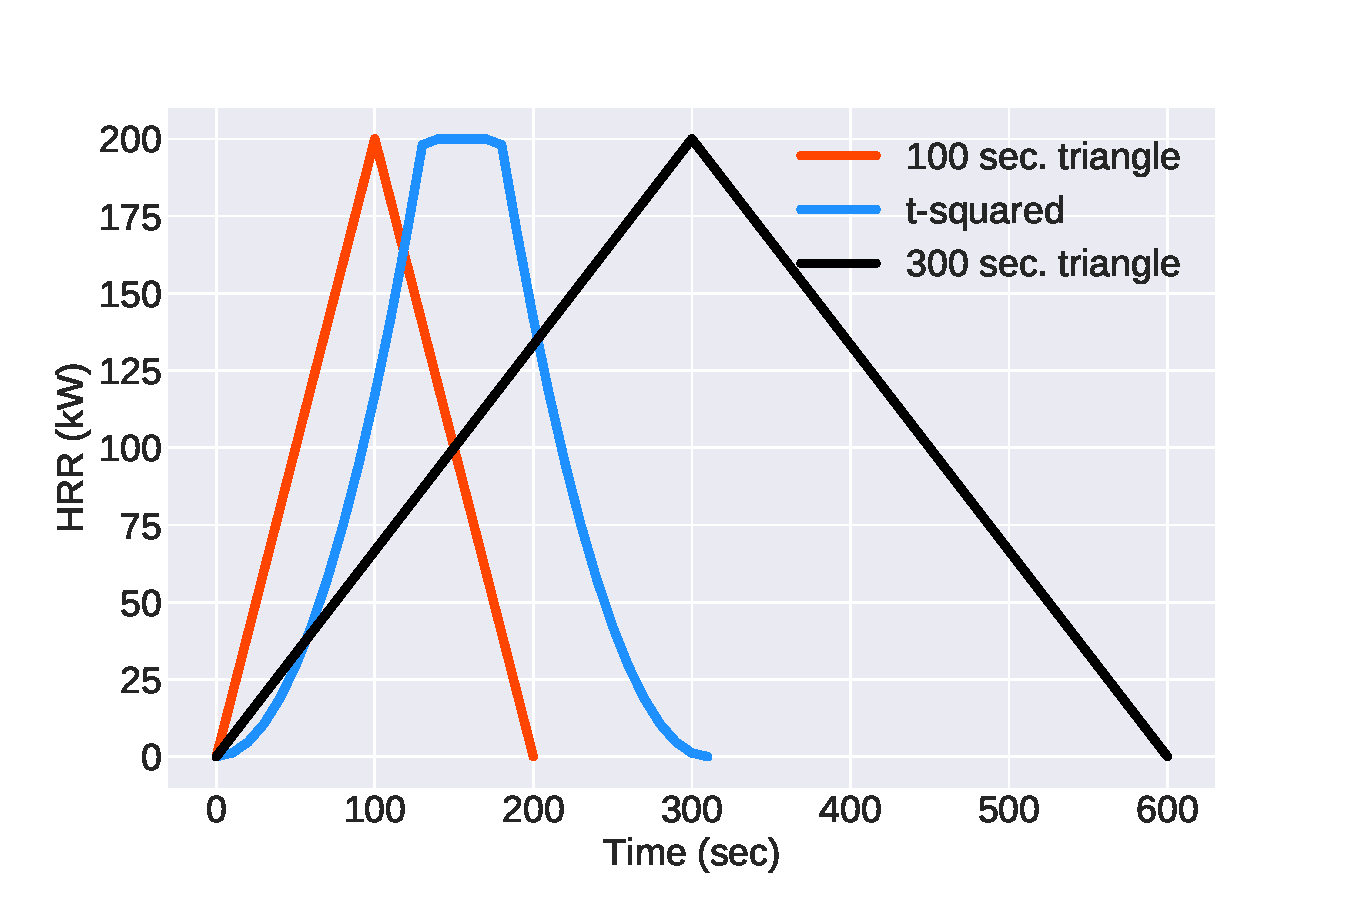
\includegraphics[width=\textwidth,keepaspectratio]{figures/training_ramps.pdf}
      \caption{Histogram of optimized bandwidths}
      \label{fig:bhist}
  \end{subfigure}
  \begin{subfigure}[t]{.45\textwidth}
      \centering
      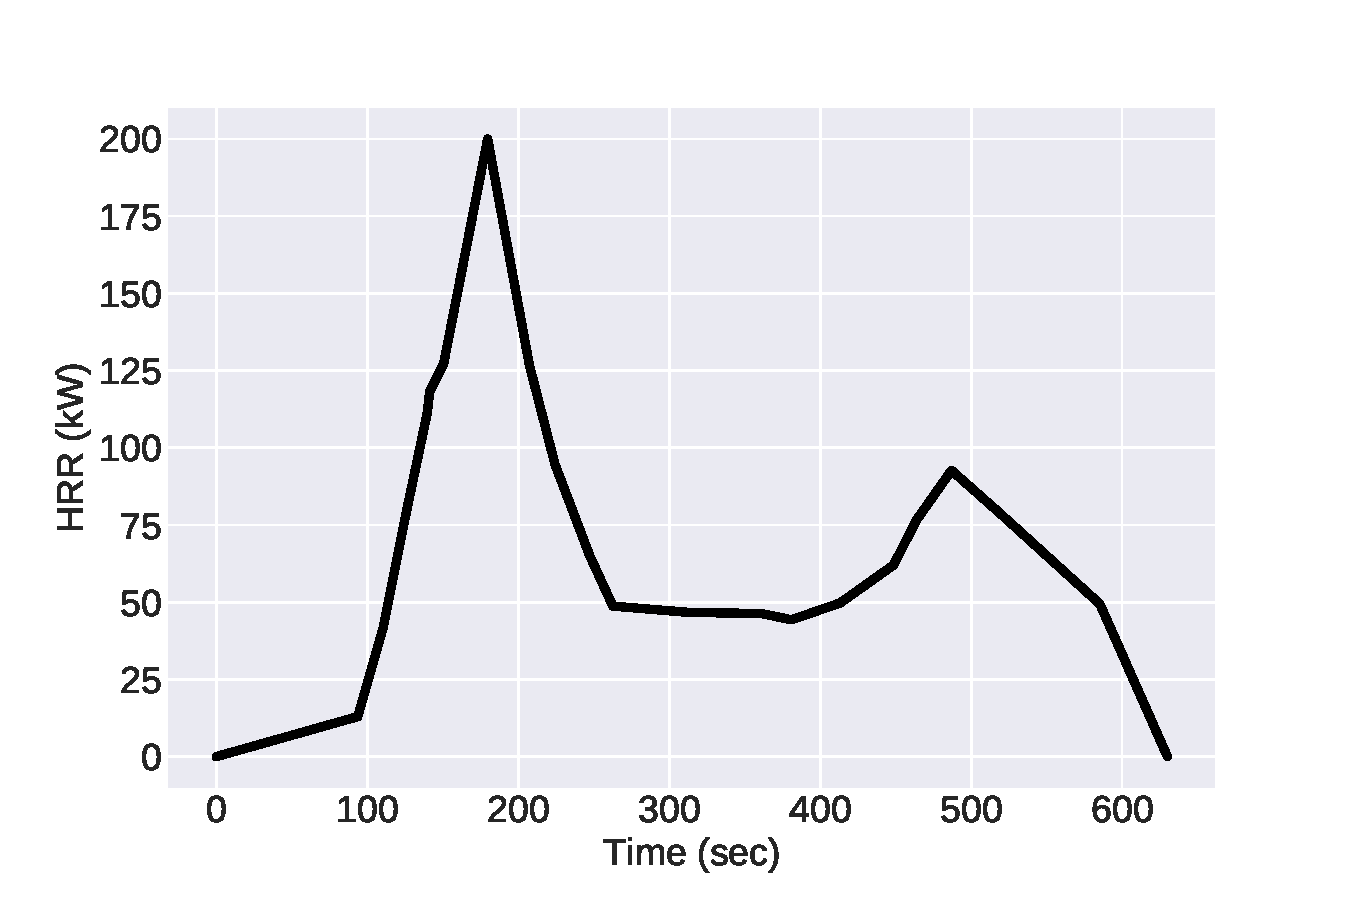
\includegraphics[width=\textwidth ,keepaspectratio]{figures/test_ramp.pdf}
      \caption{Scatterplot of optimized bandwidths vs. average department population density}
      \label{fig:popband}
  \end{subfigure}
  \caption{\protect\ref{fig:bhist} shows the variation of the optimized bandwidth across departments in the dataset, and the negative correlation apparent in \protect\subref{fig:popband} shows that this variation is at least partially explained by the variation in population density across departments.}
  \label{fig:band_optimization}
\end{figure}





\subsection{Heat flux measurements}
This section describes machine learning methods for inferring the heat release rate of a compartment fire using heat flux measurements from the directional flame thermometers (DFTs) of the aforementioned experimental setup. A simple starting point is to plot the heat release rates from the training fires against the heat fluxes measured by the DFTs. Although 34 for these scatter plots could be generated (one for each DFT in the setup), Figure 






\begin{figure}[htbp] \centering
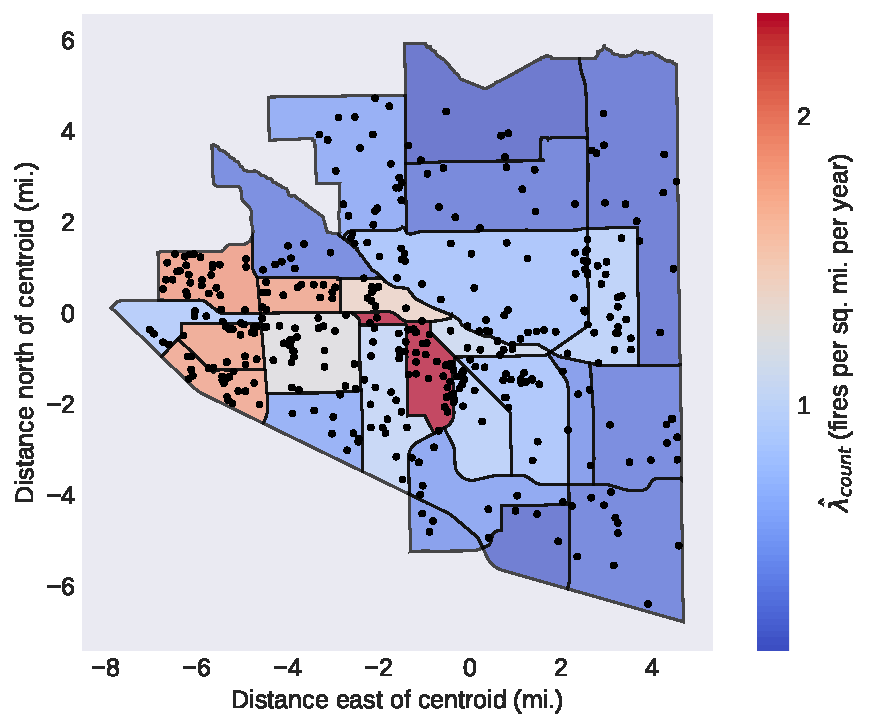
\includegraphics[width=.75\textwidth]{./figures/spatial_histogram.pdf}
\caption{A visual depiction of the naive count forecasting methodology for an example department. Each black dot marker indicates the location of a residential fire that occurred during the six-year training interval, 2006-2011 (inclusive). The color of a tract corresponds to the fire count density rate estimated from this approach for that tract. Notice that large census tracts with few fires have the lowest density rate and small tracts with many fires have the highest density rate.}
\label{fig:spatial_histogram}
\end{figure}








\clearpage
\bibliographystyle{unsrtnat}
\bibliography{./references.bib}
\end{document}
